Das System, als Web-Applikation, interagiert mit anderen Systemen in seiner Umgebung. TODO kommuniziert zur Übertragung von Daten mit mehreren Clients, welche Anfragen senden und Antworten empfangen, und mit weiteren Servern um Daten in den Datenbanken auszutauschen.\\
\begin{figure}[h]
\centering
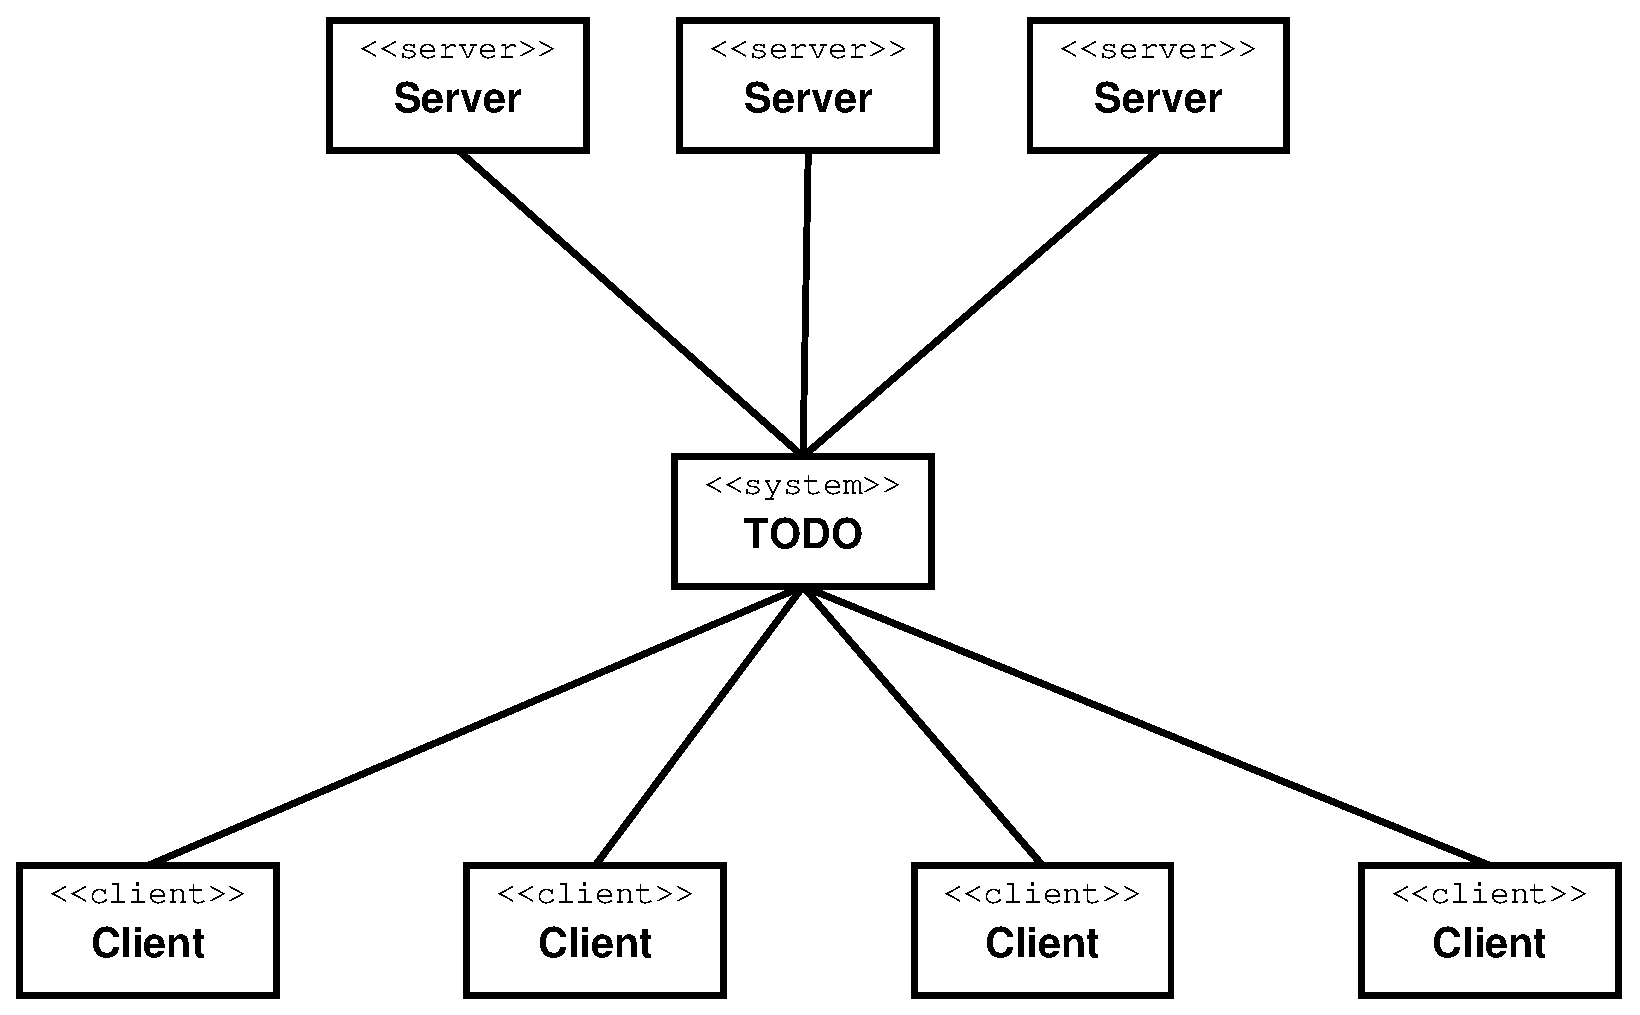
\includegraphics[width=0.9\linewidth]{Grafik/Diagramm/External}
\caption[Context Diagram]{Context Diagram des Systems im Bezug zu seiner Umgebung}
\label{fig:External}
\end{figure}\\
Die Kommunikation zwischen dem TODO und anderen Servern läuft dabei über das REST-Interface ab. Auch die Clients nutzen REST um Anfragen an das System zu stellen. Die Verbindung wird über HTTPS aufgebaut.